%%----------------------------------------------------------------------------
%% Presentatie HoGent Bedrijf en Organisatie
%%----------------------------------------------------------------------------
%% Auteur: Bert Van Vreckem [bert.vanvreckem@hogent.be]

\documentclass{beamer}

%==============================================================================
% Aanloop
%==============================================================================

%---------- Packages ----------------------------------------------------------
\usepackage{etex}
\usepackage{graphicx,multicol}
\usepackage{comment,enumerate,hyperref}
\usepackage{amsmath,amsfonts,amssymb}
\usepackage{tikz}
\usepackage[dutch]{babel}
\usepackage[utf8]{inputenc}
\usepackage{multirow}
\usepackage{eurosym}
\usepackage{listings}
\usepackage[T1]{fontenc}
\usepackage{lmodern}
\usepackage{textcomp}
\usepackage{framed}
\usepackage{wrapfig}
\usepackage{pgf-pie}
\usepackage{pgfplots}
\usepackage{booktabs}
\usepackage{pgfplotstable}
\usepackage{changepage}

%---------- Configuratie ------------------------------------------------------

\usetikzlibrary{arrows,shapes,backgrounds,positioning,shadows}
\usetikzlibrary{pgfplots.statistics}


\usetheme{hogent}
\setbeameroption{show notes}

%---------- Commando-definities -----------------------------------------------

\newcommand{\tabitem}{~~\llap{\textbullet}~~}
\renewcommand{\arraystretch}{1.2}

%---------- Info over de presentatie ------------------------------------------

\title[Intro]{Onderzoekstechnieken\\Toetsen van een hypothese}
\author{Jens Buysse \and Wim {De Bruyn} \and Wim Goedertier \and Bert {Van Vreckem}}
\date{AJ 2017-2018}

%==============================================================================
% Inhoud presentatie
%==============================================================================

\begin{document}

%---------- Front matter ------------------------------------------------------

% Dia met het HoGent logo
\HoGentLogo

% Titeldia met faculteitslogo
\titleframe

%---------- Inhoud ------------------------------------------------------------

\pgfmathdeclarefunction{gauss}{2}{%
  \pgfmathparse{1/(#2*sqrt(2*pi))*exp(-((x-#1)^2)/(2*#2^2))}%
}

\begin{frame}
  \frametitle{What's on the menu today?}

  \tableofcontents
\end{frame}

\section{Toetsen van hypothesen}
\sectionframelogo{}

\begin{frame}
  \frametitle{De statistische test voor een hypothese}

  \begin{description}
    \item[Hypothese] Idee waarvan nog bewezen moet worden dat het juist is: uitspraak over numerieke waarde van een populatieparamter
    \item[Hypothesetest] controle van een uitspraak over de waarden van één of meerdere populatieparameters
  \end{description}
\end{frame}

\begin{frame}
  \frametitle{Elementen bij toetsingsprocedure}

  \begin{description}
    \item[Nulhypothese ($H_0$)] Deze hypothese proberen we te ontkrachten door redenering in het ongerijmde
    \item[Alternatieve hypothese ($H_1$, $H_a$)] Deze hypothese willen we aantonen
    \item[Toetsingsgrootheid] De variabele die berekend wordt uit de steekproef (ook: teststatistiek)
    \item[Aanvaardingsgebied] Het gebied van waarden die de nulhypothese \emph{ondersteunt}
    \item[Kritieke of Verwerpingsgebied] Het gebied van waarden die de nulhypothese \emph{verwerpt}
  \end{description}
\end{frame}

\section{Werkwijze}
\sectionframelogo{}

\begin{frame}
  \frametitle{Werkwijze}

  \begin{enumerate}
    \item Bepalen van de hypotheses ($H_0$ en $H_a$)
    \item Vastlegen significantieniveau ($\alpha$ en $n$)
    \item Toetsingsgrootheid berekenen
    \item Het kritieke gebied of de overschrijdingskans bepalen
    \item Conclusies trekken
  \end{enumerate}
\end{frame}

\begin{frame}
  \frametitle{Hypotheses over superhelden}

  
\includegraphics[width=\textwidth]{img/les5-heroes}
\end{frame}

\begin{frame}
  \frametitle{Een superheld redt 3.3 mensen per dag}

  \begin{columns}
    \column{.5\textwidth}
    \centering
    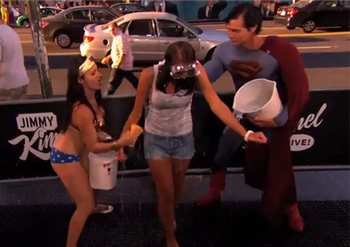
\includegraphics[width=4cm]{img/les5-gered1}

    
\includegraphics[width=4cm]{img/les5-gered2}
    \column{.5\textwidth}
    \centering
    
\includegraphics[width=4cm]{img/les5-gered3}

    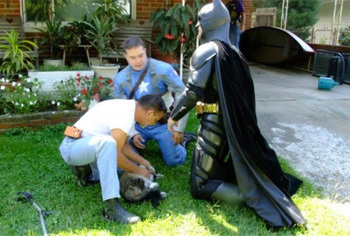
\includegraphics[width=4cm]{img/les5-gered4}
  \end{columns}

  \vfill
  \centering
  \small{Bron: \url{http://www.cracked.com/quick-fixes/4-people-who-saved-day-while-dressed-as-superheroes/}}
\end{frame}

\begin{frame}

  Stel, in een steekproef van $n = 30$ dagen werd een gemiddelde van $3.483$ reddingen gemeten.

  \begin{enumerate}
    \item Hypothese:
    
    $H_0: \mu = 3,3$; $H_1: \mu > 3,3$
    
    \item Significantieniveau $\alpha = 0,05$ en steekproefgrootte $n = 30$
    
    \item Steekproefgrootheid: $\overline{x} = 3,483$
    
    Populatiestandaardafwijking (verondersteld gekend): $\sigma = 0,55$
  \end{enumerate}
\end{frame}

\begin{frame}
  \frametitle{Berekenen toetsingsgrootheid}
  
  Uit centrale limietstelling volgt: $M \sim Nor(\mu = 3,3; \sigma = \frac{0,55}{\sqrt{30}})$

  \centering
  \begin{tikzpicture}
    \begin{axis}[domain=3.0:3.6, ymax=4.2, samples=100, enlargelimits=false ]
      \addplot [very thick,smooth,draw=HoGentFBO] {gauss(3.3, 0.10041580220928045413)};
      \node [coordinate, pin={\small{3.483}}] at (axis cs: 3.483, 0){};
    \end{axis}
  \end{tikzpicture}
\end{frame}

\section{Overschrijdingskans}
\sectionframelogo{}

\begin{frame}
  \frametitle{Overschrijdingskans}
  \brightbox{De \textcolor{HoGentAccent6}{p-waarde} is de kans, indien de nulhypothese waar is, om een waarde te verkrijgen van de toetsingsgrootheid die minstens even extreem is als de geobserveerde waarde.}

  \begin{itemize}
    \item $p$-waarde $< \alpha \Rightarrow$ $H_{0}$ verwerpen: de gevonden waarde voor $\overline{x}$ is te extreem;
    \item $p$-waarde $\geq \alpha \Rightarrow$ $H_{0}$ niet verwerpen: de gevonden waarde voor $\overline{x}$ kan nog verklaard worden door toeval.
  \end{itemize}
\end{frame}

\begin{frame}
  \frametitle{Overschrijdingskans}

  \centering
  \begin{tikzpicture}[scale=0.8]
    \begin{axis}[domain=-3.5:3.5, ymax=0.42, samples=100, enlargelimits=false, clip=false ]
      \addplot [smooth, fill=black!20, domain=1.822:3.5] {gauss(0,1)} \closedcycle;
      \addplot [very thick,smooth,draw=HoGentFBO] {gauss(0, 1)};
      \node  at (axis cs: 1.822, -.04){\small 1.822};
    \end{axis}
  \end{tikzpicture}
  
  \[ P(M > 3,483) = P \left(Z> \frac{3,483 - 3,3}{\frac{\sigma}{\sqrt{n}}}\right) = P (Z > 1,822) = 0,0344 \]
\end{frame}

\section{Kritieke gebied}
\sectionframelogo{}

\begin{frame}
  \frametitle{Kritieke gebied}
  
  \brightbox{Het \textcolor{HoGentAccent6}{kritieke gebied} is de verzameling van alle waarden voor de toetsingsgrootheid waarbij de nulhypothese kan verworpen worden.}
  
  Bepaald door grenswaarde:
  
  \[g = \mu + z \times \frac{\sigma}{\sqrt{n}} \]
  
  \begin{itemize}
    \item Links van $g$: aanvaardingsgebied ($H_0$ niet verwerpen)
    \item Rechts van $g$: kritieke gebied ($H_0$ wel verwerpen)
  \end{itemize}
  
\end{frame}


\begin{frame}
  \frametitle{Kritieke gebied normale verdeling}

  \centering
  \begin{tikzpicture}
    \begin{axis}[domain=-3.5:3.5, ymax=0.42, samples=100, enlargelimits=false, clip=false ]
      \addplot [smooth, fill=black!20, domain=1.645:3.5] {gauss(0,1)} \closedcycle;
      \addplot [very thick,smooth,draw=HoGentFBO] {gauss(0, 1)};
      \node  at (axis cs: 1.645, -.04){\small 1.645};
    \end{axis}
  \end{tikzpicture}
  
  De $z$-waarde die de grenswaarde bepaalt voor een significantieniveau $\alpha = 0,05$
\end{frame}

\begin{frame}
  \frametitle{Linkszijdig toetsen}
    Wat zou je in de verg.  moeten veranderen opdat je de correcte kritieke waarde zou berekenen?
    \pause
    Antwoord:
 \[g = \mu - z \times \frac{\sigma}{\sqrt{n}} \]
want
\[ P(M < g) = P\left(Z < \frac{g - \mu}{\frac{\sigma}{\sqrt{n}}}\right) = 0.05 \]
Wegens de symmetrieregel kunnen we zeggen
\[ P\left(Z > - \left( \frac{g - \mu}{\frac{\sigma}{\sqrt{n}}} \right) \right) = 0.05 \]
De z-waarde die ermee overeen komt is 1.645 dus hebben we
\[ z = \frac{-g + \mu}{\frac{\sigma}{\sqrt{n}}} \]
\[ \Leftrightarrow -g = \frac{\sigma}{\sqrt{n}} z - \mu \]
\[ \Leftrightarrow g = \mu - z \frac{\sigma}{\sqrt{n}} \]
\end{frame}

\begin{frame}
  \frametitle{Tweezijdig toetsen}
  Soms kan het ook zijn dat er tweezijdig moet getoetst worden. Er moeten dan twee kritieke grenswaarden berekend worden namelijk de linker- en de rechter grenswaarden.

\begin{equation}
  g = \mu \pm z \times \frac{\sigma}{\sqrt{n}}
  \label{eq:kritiekeGrenswaarde}
\end{equation}
\end{frame}

\begin{frame}
  \frametitle{Samenvatting}

\begin{table}
  \centering
  \begin{tabular}{l|ccc}
    \toprule
    Doel              & \multicolumn{3}{l}{\parbox{.7\textwidth}{Test op gemiddelde waarde $\mu$ van de populatie aan de hand van een steekproef van $n$ onafhankelijke steekproefwaarden}} \\
    \midrule
    Voorwaarde        & \multicolumn{3}{l}{\parbox{.7\textwidth}{De populatie is willekeurig verdeeld, $n$ voldoende groot}} \\
    \midrule
    Type test         & Tweezijdig           & Eenzijdig links & Eenzijdig rechts \\
    \midrule
    $H_{0}$           & $\mu = \mu_{0}$      & $\mu = \mu_{0}$ & $\mu = \mu_{0}$  \\
    $H_{1}$           & $\mu \neq \mu_{0}$   & $\mu < \mu_{0}$ & $\mu > \mu_{0}$  \\
    Verwerpingsgebied & $\left|z\right| > g$ & $z< -g $        & $z>g$            \\
    Teststatistiek    & \multicolumn{3}{c}{$z = \frac{\overline{x} - \mu_{0}}{\frac{\sigma}{\sqrt{n}}}$} \\
    \bottomrule
  \end{tabular}
  \caption{Samenvatting mogelijke toetsen}
  \label{tab:toetsingsprocedures}
\end{table}
\end{frame}

\section{Voorbeelden}
\sectionframelogo{}

\begin{frame}
  \frametitle{Voorbeeld 1}
  Bij een aselecte steekproef van 50 waarnemingen vinden we volgende grootheden: gemiddelde $\overline{x} = 25$ en standaardafwijking s = $\sqrt{55} = 7.41$
  We willen weten of er reden is om aan te nemen dat gemiddelde van de populatie kleiner is dan 27.

\end{frame}

\begin{frame}
  \frametitle{Voorbeeld 1}
  \begin{block}{Bepalen van de hypotheses}
    $H_{0} : \mu = 27$ en $H_{1}: \mu < 27$.
  \end{block}


  \begin{block}{Vastleggen significantieniveau}
  $\alpha = 0.05$ en $n=50$.
  \end{block}


  \begin{block}{Toetsingsgrootheiden \& waarde}
  We kiezen hiervoor het steekproefgemiddelde $M$. Volgens de centrale limietstelling geldt:

  \[ M \sim Nor(\mu = 27, \frac{\sigma}{\sqrt{n}}) \]
  \[ z = \frac{\overline{x} - \mu}{\frac{\sigma}{\sqrt{n}}} = \frac{25-27}{\sqrt\frac{55}{50}} \approx -1.91\]
  We vinden dus een overschrijdingskans van $0.0281$.
  \end{block}
  \end{frame}

\begin{frame}
    \begin{block}{Overschrijdingskans}
    We vinden dus een overschrijdingskans van het gemiddelde van $0.02$ wat bij een significantieniveau van 0.05 erop duidt dat we $H_{0}$ mogen verwerpen.
    \end{block}

    \begin{block}{Bereken en teken kritiek gebied}
    \[ g = \mu - z \times \frac{\sigma}{\sqrt{n}} \]
    \[ g = 27 - 1.645 \times \sqrt{\frac{\sigma}{n}} \]
    \[ g = 25.27470944 \]

    We vinden dus dat $\overline{x} < g$ en dus kunnen we $H_{0}$ verwerpen.
\end{block}

\end{frame}

\begin{frame}
    \centering
  \begin{tikzpicture}
    \begin{axis}[domain=24:30, samples=100, enlargelimits=false, clip=false ]
      \addplot [smooth, fill=cyan!20, domain=24:25.27] {gauss(27,1.048808848)} \closedcycle;
      \addplot [very thick,smooth,draw=HoGentFBO] {gauss(27, 1.048808848)};
      \node  at (axis cs: 25.27, -.04){\small 25.27};
    \end{axis}
  \end{tikzpicture}
\end{frame}

\begin{frame}
  \frametitle{Voorbeeld 2}
  In een onderzoek naar het kleingeld dat in de zakken van  van  onze superhelden zit, wordt er van uit gegaan dat ze gemiddeld \euro{25} op zak hebben. We gaan ervan uit dat we een gekende spreiding van $\sigma = 7$ hebben. Verder zijn de gegevens van de aselecte steekproef van omvang $n=64$ beschikbaar met gemiddeld zakgeld $\overline{x}$ van \euro{23}. Neem als significantieniveau $\alpha = 0.05$.
\end{frame}

\begin{frame}
  \frametitle{Voorbeeld 2}
  \begin{block}{Bepalen van de hypotheses}
  $H_{0} : \mu = 25$ en $H_{1}: \mu \neq 25$.
  \end{block}

  \begin{block}{Vastleggen significantieniveau}
  $\alpha = 0.05$ en $n=64$.
  \end{block}

  \begin{block}{Toetsingsgrootheden \& waarde}
    \[ g_{1} = \mu - z \times \frac{\sigma}{\sqrt{n}} = 23.28 \]
    \[ g_{2} = \mu + z \times \frac{\sigma}{\sqrt{n}} = 26.72 \]
    \end{block}

    \begin{block}{Bereken en teken kritiek gebied}
      We vinden dat $\overline{x}$ in het kritieke gebied (want $23 < 23.28$) ligt dus mogen we $H_{0}$verwerpen.
  \end{block}
\end{frame}

\section{De $t$-toets}
\sectionframelogo{}

\begin{frame}
  \frametitle{Veronderstellingen $z$-toets}
  
  
  \begin{itemize}
    \item De steekproef moet aselect zijn
    \item De steekproef moet voldoende groot zijn ($n \ge 30$)
    \item De variatie van de toetsingsgrootheid moet normaal verdeeld zijn
    \item We veronderstellen dat de standaardafwijking van de populatie, $\sigma$, gekend is
  \end{itemize}

  Als deze veronderstellingen niet gelden, mag je de $z$-toets niet gebruiken!
\end{frame}

\begin{frame}
  \frametitle{De $t$-toets}
  
  Bepalen kritieke grenswaarde:
  
  \[ g = \mu \pm t \times \frac{s}{\sqrt{n}} \]
  
  \begin{itemize}
    \item $t$-waarde wordt afgeleid uit de Student-$t$ verdeling, hangt af van aantal \emph{vrijheidsgraden}, $n-1$
    \item Op te zoeken in $t$-tabel of met R-functie \texttt{pt}
  \end{itemize}
  
\end{frame}

\begin{frame}
  \frametitle{Vergelijken van twee steekproeven}
  
  Is steekproefgemiddelde van twee steekproeven significant verschillend?
  
  \begin{itemize}
    \item Onafhankelijke steekproeven
    \item Gepaarde steekproeven
  \end{itemize}
\end{frame}

\begin{frame}
  \frametitle{Voorbeeld}
  \framesubtitle{Onafhankelijke steekproeven}
  
  In een klinisch onderzoek wil men nagaan of een nieuw medicijn als bijwerking een verminderde reactiesnelheid heeft.
  
  \begin{itemize}
    \item Interventiegroep: 6 deelnemers krijgen medicijn
    \item Controlegroep: 6 deelnemers krijgen placebo
  \end{itemize}
  
  Vervolgens wordt reactiesnelheid gemeten:
  
  \begin{itemize}
    \item Controlegroep: 91, 87, 99, 77, 88, 91
    \item Interventiegroep: 101, 110, 103, 93, 99, 104
  \end{itemize}
  
  Zijn er significante verschillen tussen de interventie- en controlegroep?
\end{frame}

\begin{frame}[fragile]
  \frametitle{Voorbeeld}
  \framesubtitle{Onafhankelijke steekproeven}

\footnotesize
\begin{verbatim}
> controle <-  c(91, 87, 99, 77, 88, 91)
> interventie <- c(101, 110, 103, 93, 99, 104)
> t.test(controle, interventie, alternative="less", mu=0)

Welch Two Sample t-test

data:  controle and interventie
t = -3.4456, df = 9.4797, p-value =
0.003391
alternative hypothesis: true difference in means is less than 0
95 percent confidence interval:
-Inf -6.044949
sample estimates:
mean of x mean of y 
88.83333 101.66667
\end{verbatim}
\end{frame}


\begin{frame}
  \frametitle{Voorbeeld}
  \framesubtitle{Gepaarde steekproef}
  
  In een studie werd nagegaan of auto's die rijden op benzine met additieven ook een lager verbruik hebben.
  
  Bij 10 auto's werd het verbruik gemeten (uitgedrukt in mijl per gallon) voor beide soorten benzine:
  
  \vspace{.5cm}
  \centering
  \begin{tabular}{|l|c|c|c|c|c|c|c|c|c|c|}
  	\hline
  	Auto           & 1  & 2  & 3  & 4  & 5  & 6  & 7  & 8  & 9  & 10 \\ \hline
  	Gewone benzine & 16 & 20 & 21 & 22 & 23 & 22 & 27 & 25 & 27 & 28 \\ \hline
  	Met additieven & 19 & 22 & 24 & 24 & 25 & 25 & 25 & 26 & 28 & 32 \\ \hline
  \end{tabular} 
\end{frame}

\begin{frame}[fragile]
  \frametitle{Voorbeeld}
  \framesubtitle{Gepaarde steekproef}
  
\footnotesize
\begin{verbatim}
> gewone    <- c(16, 20, 21, 22, 23, 22, 27, 25, 27, 28)
> additieven <-c(19, 22, 24, 24, 25, 25, 26, 26, 28, 32)
> t.test(additieven, gewone, alternative="greater", paired=TRUE)

Paired t-test

data:  additieven and gewone
t = 4.4721, df = 9, p-value = 0.0007749
alternative hypothesis: true difference in means is greater than 0
95 percent confidence interval:
1.180207      Inf
sample estimates:
mean of the differences 
2
\end{verbatim}
\end{frame}

\section{Fouten in hypothesetoetsen}
\sectionframelogo{}

\begin{frame}
  \frametitle{Fouten in hypothesetoetsen}

  \begin{table}
    \centering
    \resizebox{\textwidth}{!}{%
      \begin{tabular}{@{}l|cc@{}}
        \toprule
        & \multicolumn{2}{c}{\textbf{Werkelijke stand van zaken}} \\
        \textbf{Conclusies}          & \textbf{$H_{0}$ correct} & \textbf{$H_{1}$ correct}     \\
        \midrule
        \textbf{$H_{0}$ geaccepteerd}& Juist                    & Fout van type II \\
        \textbf{$H_{0}$ verworpen}   & Fout van type I          & Juist            \\
        \bottomrule
      \end{tabular}
    }
    \caption{Mogelijke fouten bij het trekken van conclusies uit statistische toetsen.}
    \label{tab:hypfouten}
  \end{table}
\end{frame}
\end{document}
